\documentclass[tikz,border=5mm,12pt]{standalone}

\newcommand\width{22mm}
\newcommand\sep{3mm}
\newcommand\labely{-11pt-5mm}

\begin{document}
  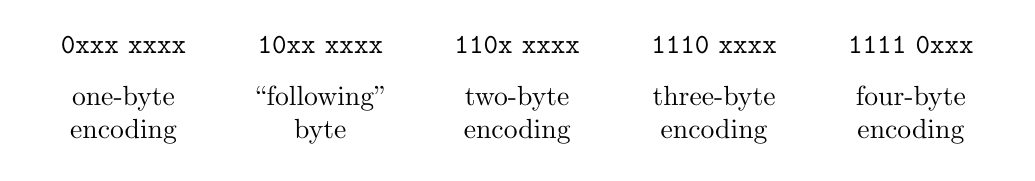
\begin{tikzpicture}
    \node[text width=\width,align=center] at (0,0) {\texttt{0xxx xxxx}};
    \node[text width=\width,align=center] at (\width+\sep,0) {\texttt{10xx xxxx}};
    \node[text width=\width,align=center] at (2*\width+2*\sep,0) {\texttt{110x xxxx}};
    \node[text width=\width,align=center] at (3*\width+3*\sep,0) {\texttt{1110 xxxx}};
    \node[text width=\width,align=center] at (4*\width+4*\sep,0) {\texttt{1111 0xxx}};

    \node[text width=\width,align=center] at (0,\labely) {one-byte\\ encoding};
    \node[text width=\width,align=center] at (\width+\sep,\labely) {``following''\\ byte};
    \node[text width=\width,align=center] at (2*\width+2*\sep,\labely) {two-byte\\ encoding};
    \node[text width=\width,align=center] at (3*\width+3*\sep,\labely) {three-byte\\ encoding};
    \node[text width=\width,align=center] at (4*\width+4*\sep,\labely) {four-byte\\ encoding};
  \end{tikzpicture}
\end{document}
